\documentclass{ustb-thesis}

% \syntaxonly

\usepackage{graphicx}

% 论文基本信息
\newcommand{\ctitlefirst}{基于模糊测试的RISC-V}  % 中文标题第一行
\newcommand{\ctitlesecond}{SBI系统测试框架研究}  % 中文标题第二行
\newcommand{\etitlefirst}{A Research Based on XXXXX}  % 英文标题第一行
\newcommand{\etitlesecond}{XXXX System Research}  % 英文标题第二行
\newcommand{\collage}{计算机与通信工程学院}  % 学院
\newcommand{\class}{物联212}  % 班级
\newcommand{\name}{王诺贤}  % 作者
\newcommand{\id}{U202141934}  % 学号
\newcommand{\firstmentorname}{XXX}  % 第一指导老师姓名
\newcommand{\firstmentortitle}{教授}  % 第一指导老师职称
\newcommand{\scondmentorname}{XXX}  % 第二指导老师姓名
\newcommand{\scondmentortitle}{副教授}  % 第二指导老师职称
\renewcommand{\year}{2025}  % 年份
\renewcommand{\month}{05}  % 月份
\newcommand{\miji}{公开}  % 密级


\begin{document}
\pagenumbering{gobble}
\begin{titlepage}
  \noindent
\includegraphics[width=0.48\textwidth]{imgs/logo.png}

  \begin{flushright}
    {\songti\zihao{5}密级:\uline{\makebox[2cm][c]{公开}}}
  \end{flushright}

  \vspace{3cm}

  {\noindent\heiti\zihao{-0}本科生毕业设计(论文)}

  \vspace{4.5cm}

  \zihao{-3}

  {\heiti 题\hspace{0.5em}目:}\uline{\makebox[7.5cm][c]{\ctitlefirst}}

  \vspace{0.4cm}

  {\heiti \hspace{3.5em}}\uline{\makebox[7.5cm][c]{\ctitlesecond}}

  \vspace{0.4cm}

  {\heiti 作\hspace{0.5em}者:}\uline{\makebox[7.5cm][c]{\name}}

  \vspace{0.4cm}

  {\heiti 学\hspace{0.5em}号:}\uline{\makebox[7.5cm][c]{\id}}

  \vspace{0.4cm}

  {\heiti 学\hspace{0.5em}院:}\uline{\makebox[7.5cm][c]{\collage}}

  \vspace{0.4cm}

  {\heiti 专\hspace{0.5em}业:}\uline{\makebox[7.5cm][c]{\major}}

  \vspace{0.4cm}

  {\heiti 成\hspace{0.5em}绩:}\uline{\makebox[7.5cm][c]{}}

  \vspace{0.7cm}

  \begin{center}
    {\songti\zihao{4}\year\ 年\ \month\ 月}
  \end{center}

\end{titlepage} 

\cleardoublepage

\begin{titlepage}
  
\begin{tikzpicture}[remember picture, overlay]
  % ---- 1. 绘制双线边框 ----
  \draw[double, line width=1pt, double distance=1pt]
      ($(current page.north west)+(3cm,-3cm)$) rectangle 
      ($(current page.south east)+(-1cm,3cm)$);

  % ---- 2. 在指定位置插入文字 ----
  \node at ($(current page.center)+(1cm,6.5cm)$) {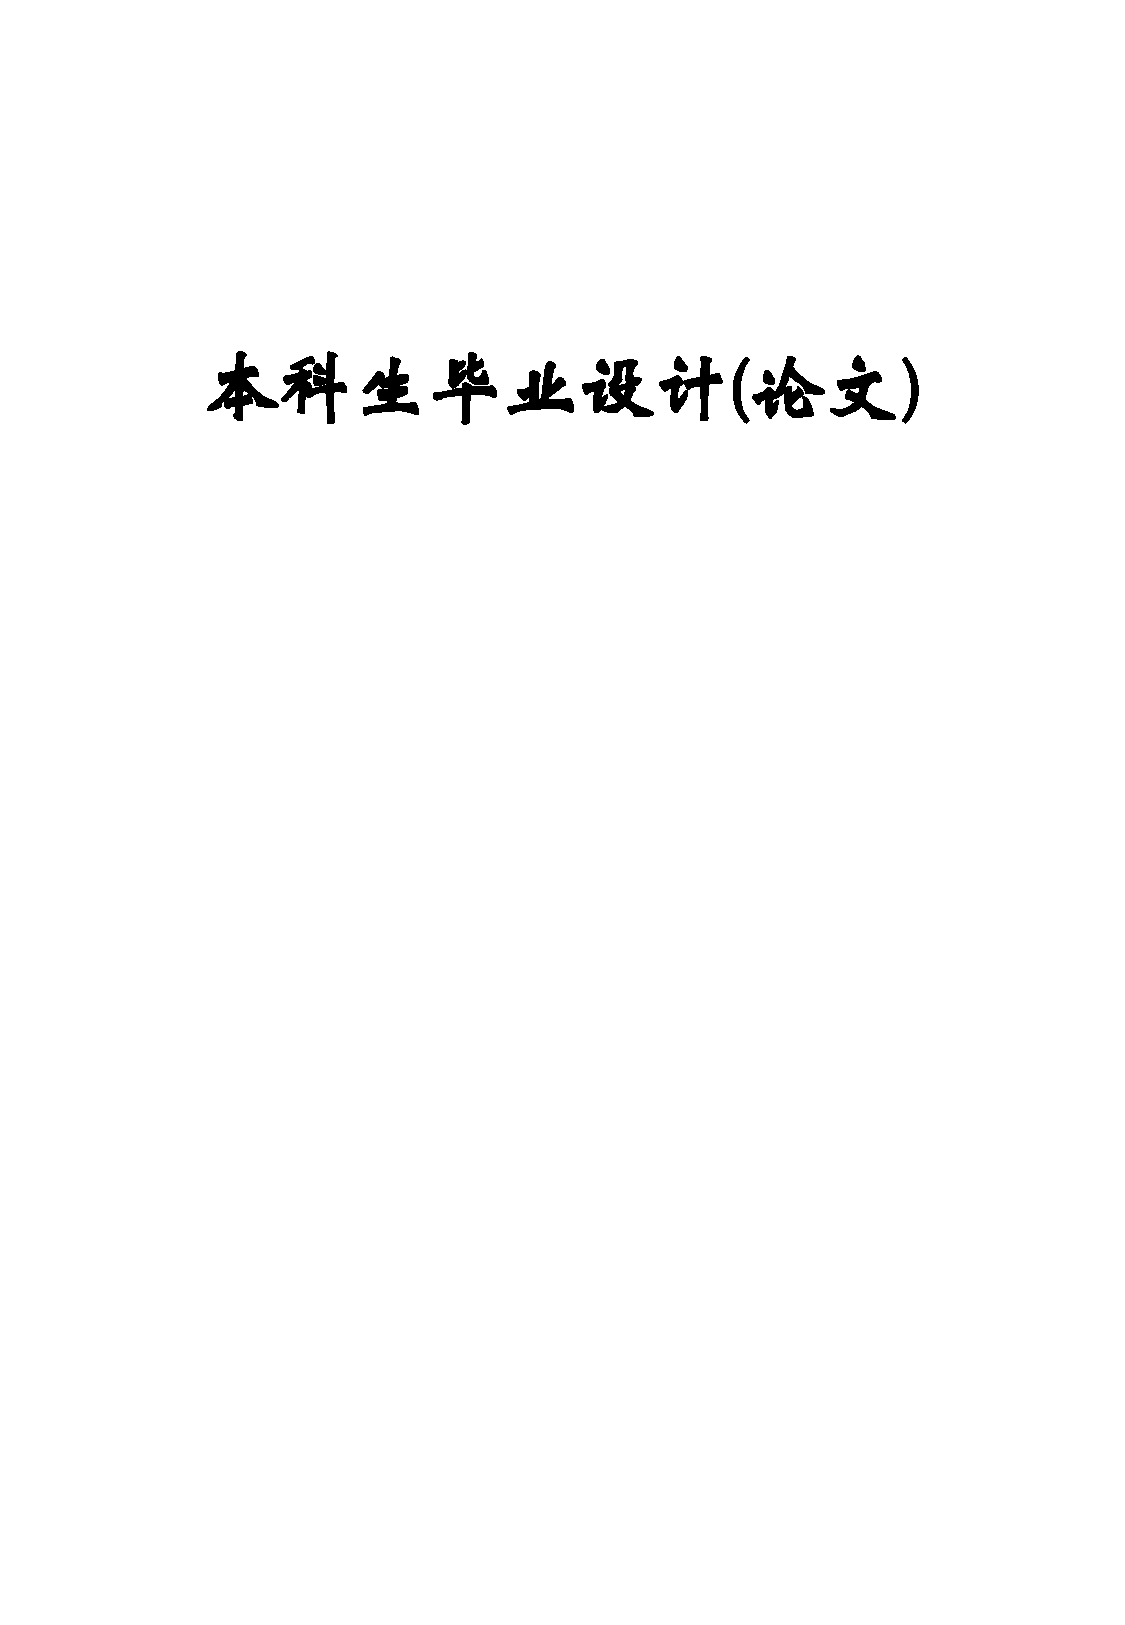
\includegraphics{imgs/title.pdf}};
  \node[align=center, font=\heiti\zihao{-3}\bfseries\selectfont] 
      at ($(current page.center)+(1.5cm,2cm)$) {
        题\hspace{2em}目:\songti\mdseries\uline{\makebox[7cm]{\ctitlefirst}}
      };
  \node[align=center, font=\heiti\zihao{-3}\bfseries\selectfont] 
      at ($(current page.center)+(1.5cm,0.7 0cm)$) {
        \hspace{5em}\songti\mdseries\uline{\makebox[7cm]{\ctitlesecond}}
      };
  \node[align=center, font=\heiti\zihao{-3}\bfseries\selectfont] 
      at ($(current page.center)+(1.5cm,-0.6cm)$) {
        英文题目:\songti\mdseries\uline{\makebox[7cm]{\etitlefirst}}
      };
  \node[align=center, font=\heiti\zihao{-3}\bfseries\selectfont] 
      at ($(current page.center)+(1.5cm,-1.9cm)$) {
        \hspace{5em}\songti\mdseries\uline{\makebox[7cm]{\etitlesecond}}
      };
  \node[align=center, font=\heiti\zihao{-3}\bfseries\selectfont] 
      at ($(current page.center)+(1.5cm,-3.2cm)$) {
        学\hspace{2em}院:\songti\mdseries\uline{\makebox[7cm]{\collage}}
      };
  \node[align=center, font=\heiti\zihao{-3}\bfseries\selectfont] 
      at ($(current page.center)+(1.5cm,-4.5cm)$) {
        班\hspace{2em}级:\songti\mdseries\uline{\makebox[7cm]{\class}}
      };
  \node[align=center, font=\heiti\zihao{-3}\bfseries\selectfont] 
      at ($(current page.center)+(1.5cm,-5.8cm)$) {
        学\hspace{2em}生:\songti\mdseries\uline{\makebox[7cm]{\name}}
      };
  \node[align=center, font=\heiti\zihao{-3}\bfseries\selectfont] 
      at ($(current page.center)+(1.5cm,-7.1cm)$) {
        学\hspace{2em}号:\songti\mdseries\uline{\makebox[7cm]{\id}}
      };
  \node[align=center, font=\heiti\zihao{-3}\bfseries\selectfont] 
      at ($(current page.center)+(1.5cm,-8.4cm)$) {
        指导教师:\songti\mdseries\uline{\makebox[2.6cm]{\firstmentorname}}
        \heiti\bfseries 职称:\songti\mdseries\uline{\makebox[2.65cm]{\firstmentortitle}}
      };
  \node[align=center, font=\heiti\zihao{-3}\bfseries\selectfont] 
      at ($(current page.center)+(1.5cm,-9.7cm)$) {
        指导教师:\songti\mdseries\uline{\makebox[2.6cm]{\secondmentorname}}
        \heiti\bfseries 职称:\songti\mdseries\uline{\makebox[2.65cm]{\secondmentortitle}}
      };

\end{tikzpicture}
\end{titlepage} 

\cleardoublepage


{\centering\chapter*{声\hspace{2em}明}}
{
  \songti\zihao{4}\linespread{2.1}\selectfont
  本人郑重声明:所呈交的论文是本人在指导教师的指导下进行的研究工作及取得研究结果。论文在引用他人已经发表或撰写的研究成果时,已经作了明确的标识;除此之外,论文中不包括其他人已经发表或撰写的研究成果,均为独立完成。其他同志对本文所做的任何贡献均已在论文中做了明确的说明并表达了谢意。\par

  \vspace{4.5cm}

  \begin{flushright}
  
  学生签名:\uline{\makebox[3cm]{}}\hspace{1.5em}\uline{\makebox[4em]{}}年\uline{\makebox[1.5em]{}}月\uline{\makebox[1.5em]{}}日

  \vspace{2cm}

  导师签名:\uline{\makebox[3cm]{}}\hspace{1.5em}\uline{\makebox[4em]{}}年\uline{\makebox[1.5em]{}}月\uline{\makebox[1.5em]{}}日

  \end{flushright}
}

\cleardoublepage

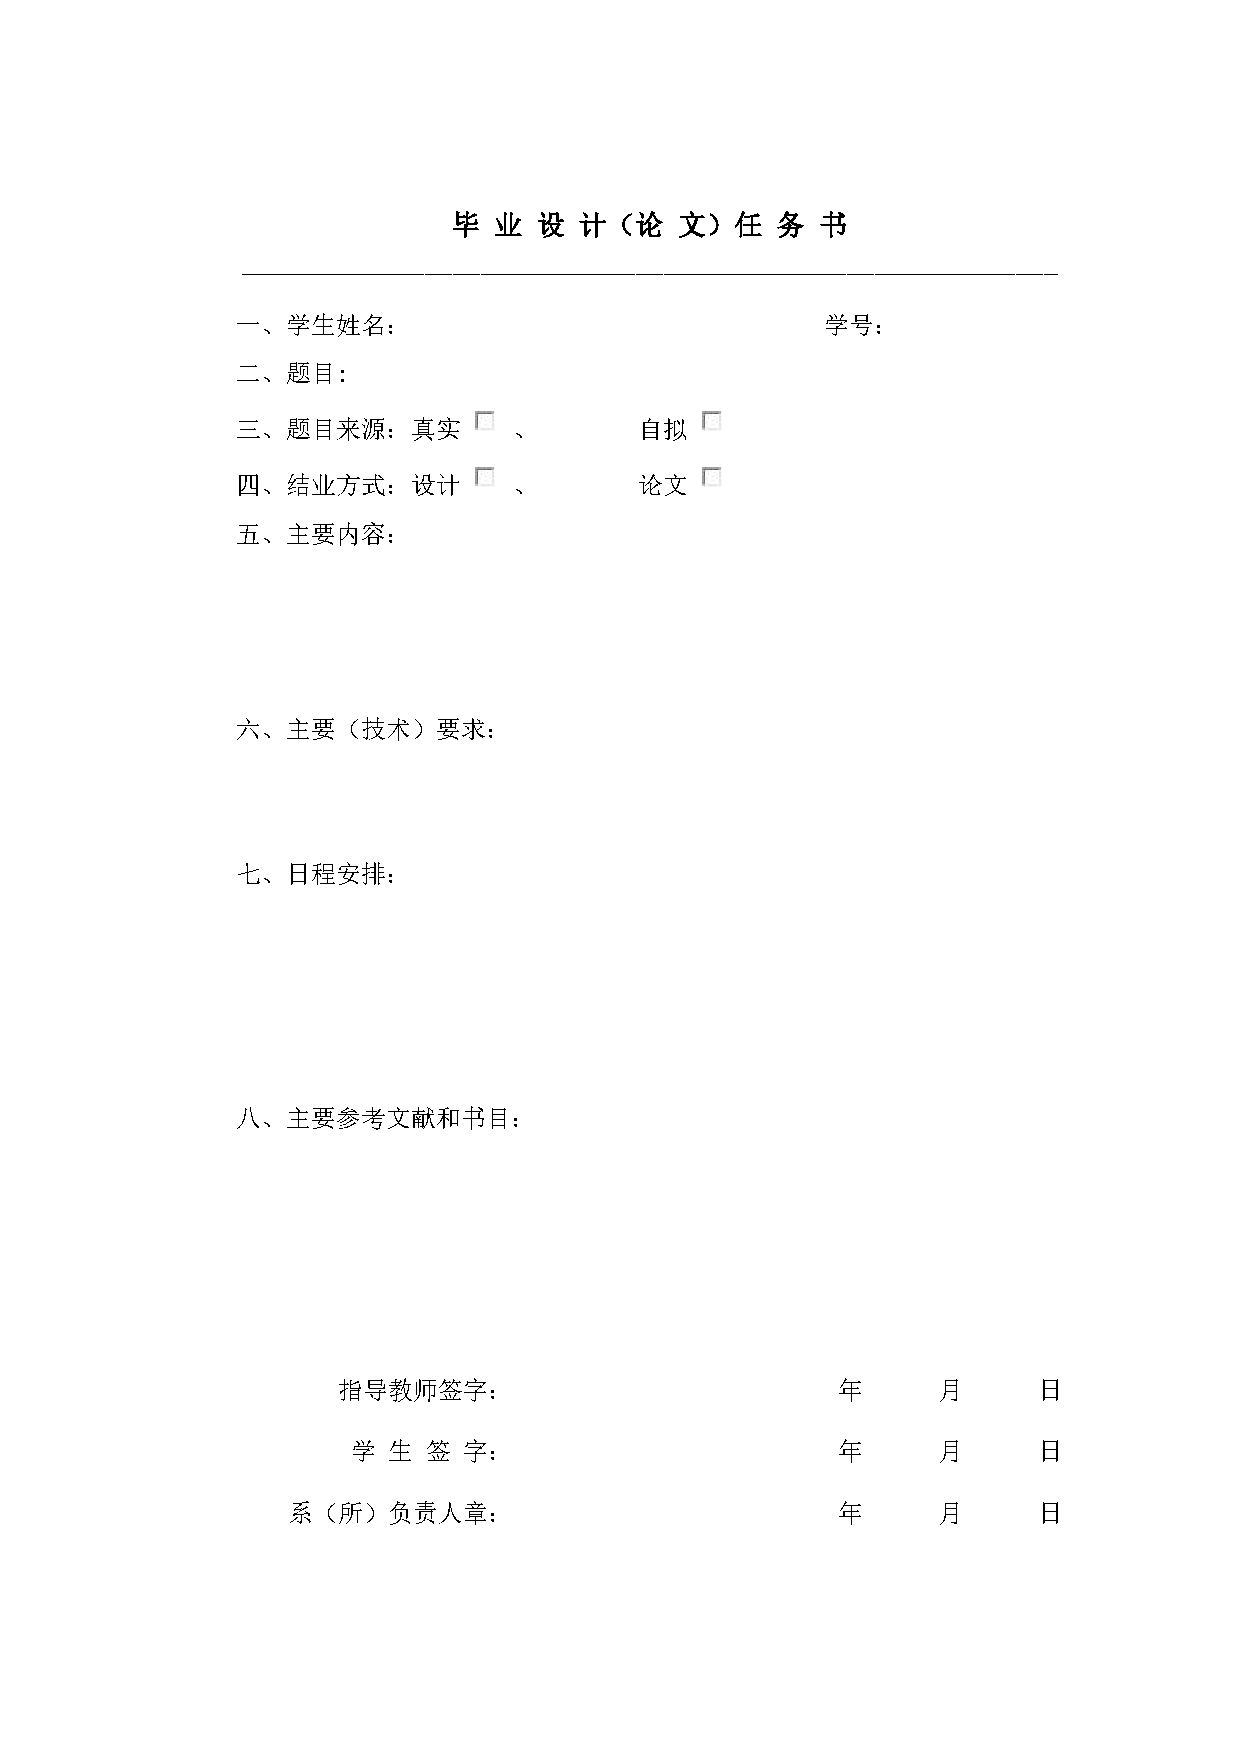
\includepdf[pages=-]{src/4-taskplan.pdf}

\cleardoublepage

\pagenumbering{Roman}

\addcontentsline{toc}{chapter}{摘\hspace{1em}要}


{\centering\chapter*{摘\hspace{1em}要}}

% 中文摘要

这是一段很长很长很长很长很长很长很长很长很长很长很长很长很长很长很长很长很长很长很长很长很长很长很长很长很长很长很长很长很长很长很长很长很长很长很长很长很长很长很长很长很长很长很长很长很长很长很长很长很长很长很长很长很长很长很长很长很长很长很长很长很长很长很长很长很长很长很长很长很长很长很长很长很长很长很长很长很长很长很长很长很长很长很长很长很长很长很长很长很长很长很长很长很长很长很长很长很长很长很长很长很长很长很长很长很长很长很长很长很长很长很长很长很长很长很长很长很长很长很长很长很长很长很长很长很长很长很长很长很长很长很长很长很长很长很长很长很长很长很长很长很长很长很长很长很长很长很长很长很长很长很长很长很长很长很长很长很长很长很长很长很长很长很长很长很长很长很长很长很长很长很长很长很长很长很长很长很长很长很长很长很长很长很长很长很长很长很长很长很长很长很长很长很长很长很长很长很长很长很长很长很长很长很长很长很长很长很长很长很长很长很长很长很长很长很长很长很长很长很长很长很长很长很长很长很长很长很长很长很长很长很长很长很长很长很长很长很长很长很长很长很长很长很长很长很长很长很长很长很长很长很长很长很长很长很长很长很长很长很长很长很长很长很长很长很长很长很长很长很长很长很长很长很长很长很长很长很长很长很长很长很长很长很长很长很长很长很长很长很长很长很长很长很长很长很长很长很长很长很长很长很长很长很长很长很长很长很长很长很长很长很长很长很长很长很长很长很长很长很长很长很长很长很长很长很长很长很长很长很长很长很长很长很长很长很长很长很长很长很长很长很长很长很长很长很长很长很长很长很长很长很长很长很长很长很长很长很长很长很长很长很长很长很长很长很长很长很长很长很长很长很长很长很长很长很长很长很长很长很长很长很长很长很长很长很长很长很长很长很长很长很长很长很长很长很长很长很长很长很长很长很长很长很长很长很长很长很长很长很长很长很长很长很长很长很长很长很长很长很长很长很长很长很长很长很长很长很长很长很长很长很长很长很长很长很长很长很长很长很长很长很长很长很长很长很长很长很长很长很长很长很长很长很长很长很长很长很长很长很长很长很长很长很长很长很长很长很长很长很长很长很长很长很长很长很长很长很长很长很长很长很长很长很长很长很长很长很长很长很长很长很长很长很长很长很长很长很长很长很长很长很长很长很长很长很长很长很长很长很长很长很长很长很长很长很长很长很长很长很长很长很长很长很长很长很长很长很长很长很长很长很长很长很长很长很长很长很长很长很长很长很长很长很长很长很长很长很长很长很长很长很长很长很长很长很长很长很长很长很长很长很长很长很长很长很长很长很长很长很长很长很长很长很长很长很长很长很长很长很长很长很长很长很长很长很长很长很长很长很长很长很长很长很长很长很长很长很长很长很长很长很长很长很长很长很长很长很长很长很长很长很长很长很长很长很长很长很长很长很长很长很长很长很长很长很长很长很长很长很长很长很长很长很长很长很长很长很长很长很长很长很长很长很长很长很长很长很长很长很长很长很长很长很长很长很长很长很长很长很长很长很长很长很长很长很长很长很长很长很长很长很长很长很长很长很长很长很长很长很长很长很长很长很长很长很长很长很长很长很长很长很长很长很长很长很长很长很长很长很长很长很长的文字。

\vfill

{
  \heiti\zihao{-4}\bfseries 关键词:\ckeywords
}

\vspace{3cm}

\cleardoublepage

\addcontentsline{toc}{chapter}{Abstract}

{\centering\chapter*{\etitlefirst\ \etitlesecond}}

{\centering\heiti\zihao{-3}\selectfont\bfseries Abstract\par}

\vspace{27pt}

% 英文摘要

This is a very very very very very very very very very very very very very very very very very very very very very very very very very very very very very very very very very very very very very very very very very very very very very very very very very very very very very very very very very very very very very very very very very very very very very very very very very very very very very very very very very very very very very very very very very very very very very very very very paragraph.

\vfill

{
  \heiti\zihao{-4}\bfseries Keywords: \ekeywords
}

\vspace{3cm}


\cleardoublepage

\tableofcontents

\cleardoublepage

\pagenumbering{arabic}
\chapter{第一章}
\section{第一节}
\subsection{第一小节}
中文测试中文测试中文测试中文测试中文测试中文测试中文测试中文测试中文测试中文测试中文测试中文测试中文测试中文测试中文测试中文测试中文测试中文测试中文测试中文测试中文测试

中文测试中文测试中文测试中文测试中文测试中文测试中文测试中文测试中文测试中文测试中文测试中文测试中文测试中文测试中文测试中文测试中文测试中文测试中文测试中文测试中文测试
\section{第一节}

\section{第一节}
\section{第一节}
\section{第一节}
\section{第一节}
\section{第一节}
\end{document}

